\chapter{Lower bound of the "shortest path in the plane with polygonal obstacles" problem}
\label{chapter:lowerbound}
In this chapter we will show the shortest path without violation has a
$\Omega{(n\log n)}$ lower bound in the algebraic computation tree model,
therefore affirming that the Hershberger Suri algorithm is optimal.  After
defining the algebraic computation tree model, we firstly introduce the element
distinction problem, then we present a lower bound for that problem.
Afterwards,
we present the sorting problem, and we make a reduction to the element
distinction problem and thereby showing, that sorting must have at least the
same lower bound as element distinction and lastly showing that the shortest
path in the plane without violations can be used to sort number and thereby
showing that the shortest path problem has a lower bound which is at least the
same.
\section{The algebraic computation tree model}
This section is based on \cite{DBLP:conf/stoc/Ben-Or83}.
The idea of the The Algebraic Computation Tree Model is to construct a rooted
tree where each path from the root to a leaf is a membership test.
Let $W \subseteq \mathbb{R}^n$ be any set. The membership problem for $W$ is
the following:
\begin{align}
	\text{Given } x = (x_1,\dots,x_n) \in \mathbb{R}^n \text{ determine if } x\in W
\end{align}
Formally a computation tree $T$ for each vertex $v$ it holds that
\begin{itemize}
  \item If $v$ has one son it computes one of the following computations
			\begin{align}
				f_v:=f_{v_1} \circ f_{v_2}\quad \text{ or }\quad
				f_v:=c \circ f_{v_1}\quad \text{ or }\quad
				f_v:=\sqrt{f_{v_1}}
				\label{form:computation}
			\end{align}
  	 where $v_i$ is an ancestor of $v$ in the tree $T$ or $f_{v_i}\in
  	 \{x_1,\dots,x_n\}$, $\circ \in \{+,-,\cdot,/\}$
   \item If $v$ has two children it is a test instruction on the form
		\begin{align}
			 f_{v_1}>0\quad \text{ or }\quad
			 f_{v_1}\geq 0\quad \text{ or }\quad
			 f_{v_1}= 0
			 \label{form:comparison}
		\end{align}
   \item If $v$ is a leaf it is either labeled YES or NO, depending on
  	 weather the path down the tree $T$ makes $(x_1,\dots,x_n)\in W$
\end{itemize}
So given an input $x\in \mathbb{R}^n$ we can build a tree $T$ and find the
depth of the tree to see what the lower bound of the computation is.
The important thing to note is that we are allowed to make comparisons (formula
\ref{form:comparison}) and computations (formula \ref{form:comparison}).

\section{Element distinction problem}

The element distinctness problem is as follows
\begin{mydef} \textbf{(Element distinctness problem:)} \\
	\label{def:distinction}
	Given $n$ elements $x_1,\dots,x_n\in \mathbb{R}$ is there a pair $x_i=x_j$
	where $i\neq j$?
\end{mydef}

The following theorem is due to Michael Ben-Or 1983 \cite{DBLP:conf/stoc/Ben-Or83}

\begin{theorem}
	\label{thm:distinction_lower}
Any algebraic computation tree that solves the n-element distinctness problem
must have complexity of at least $\Omega{(n \log n)}$
\end{theorem}

With that settled, we will move on to sorting.

\subsection{Sorting of numbers}

\begin{mydef}[Section 2.1 \cite{IntroToAlg}]\textbf{(Sorting:)} \label{def:sorting} \\
    Given a sequence of $n$ numbers $x_1,\dots,x_n$ find er permutation
	$x'_1,\dots,x'_n$ such that  $x'_1\leq x'_2 \leq\dots\leq x'_n$
\end{mydef}

Now we make a reduction from distinction problem (Definition \ref{def:distinction}) to
the sorting problem (Definition \ref{def:sorting}). We are given $x_1,\dots,
x_n$, and would like to
see if there exists a pair $x_i=x_j$ where $i\neq j$. We do this by sorting the
values and afterwards make a linear scan to see if $x'_i = x'_{i+1}$ since the 
elements is in sorted order, two element that are the same will appear next to
each other in the sorted sequence, so we will find it using this approach.
Since the reduction takes $O(n)$ and the element distinction can be solved
using sorting that means that sorting must have at least the same lower bound,
$\Omega(n\log n)$, as element distinction. 

\subsection{Shortest path in the plane}
Now we make a reduction from sorting numbers to calculating the shortest path
in the plane with obstacles (See section \ref{problemdescription} for the
formal definition).
Given numbers $x_1,\dots,x_n\in \mathbb{N}$, and let us for simplicity say that they
are all positive
(i.e.\ $x_i>0$ for $i=1,\dots,n$) we construct the obstacle as follows: Take each
point $x_i$ and construct a rectangle with the following points
$(x_i,x_i^2),(x_i-1,x_i^2),(x_i-1,\max), (x_i,\max)$, where max is the maximum
value (see Figure \ref{fig:reduction})

\begin{figure}[H]
	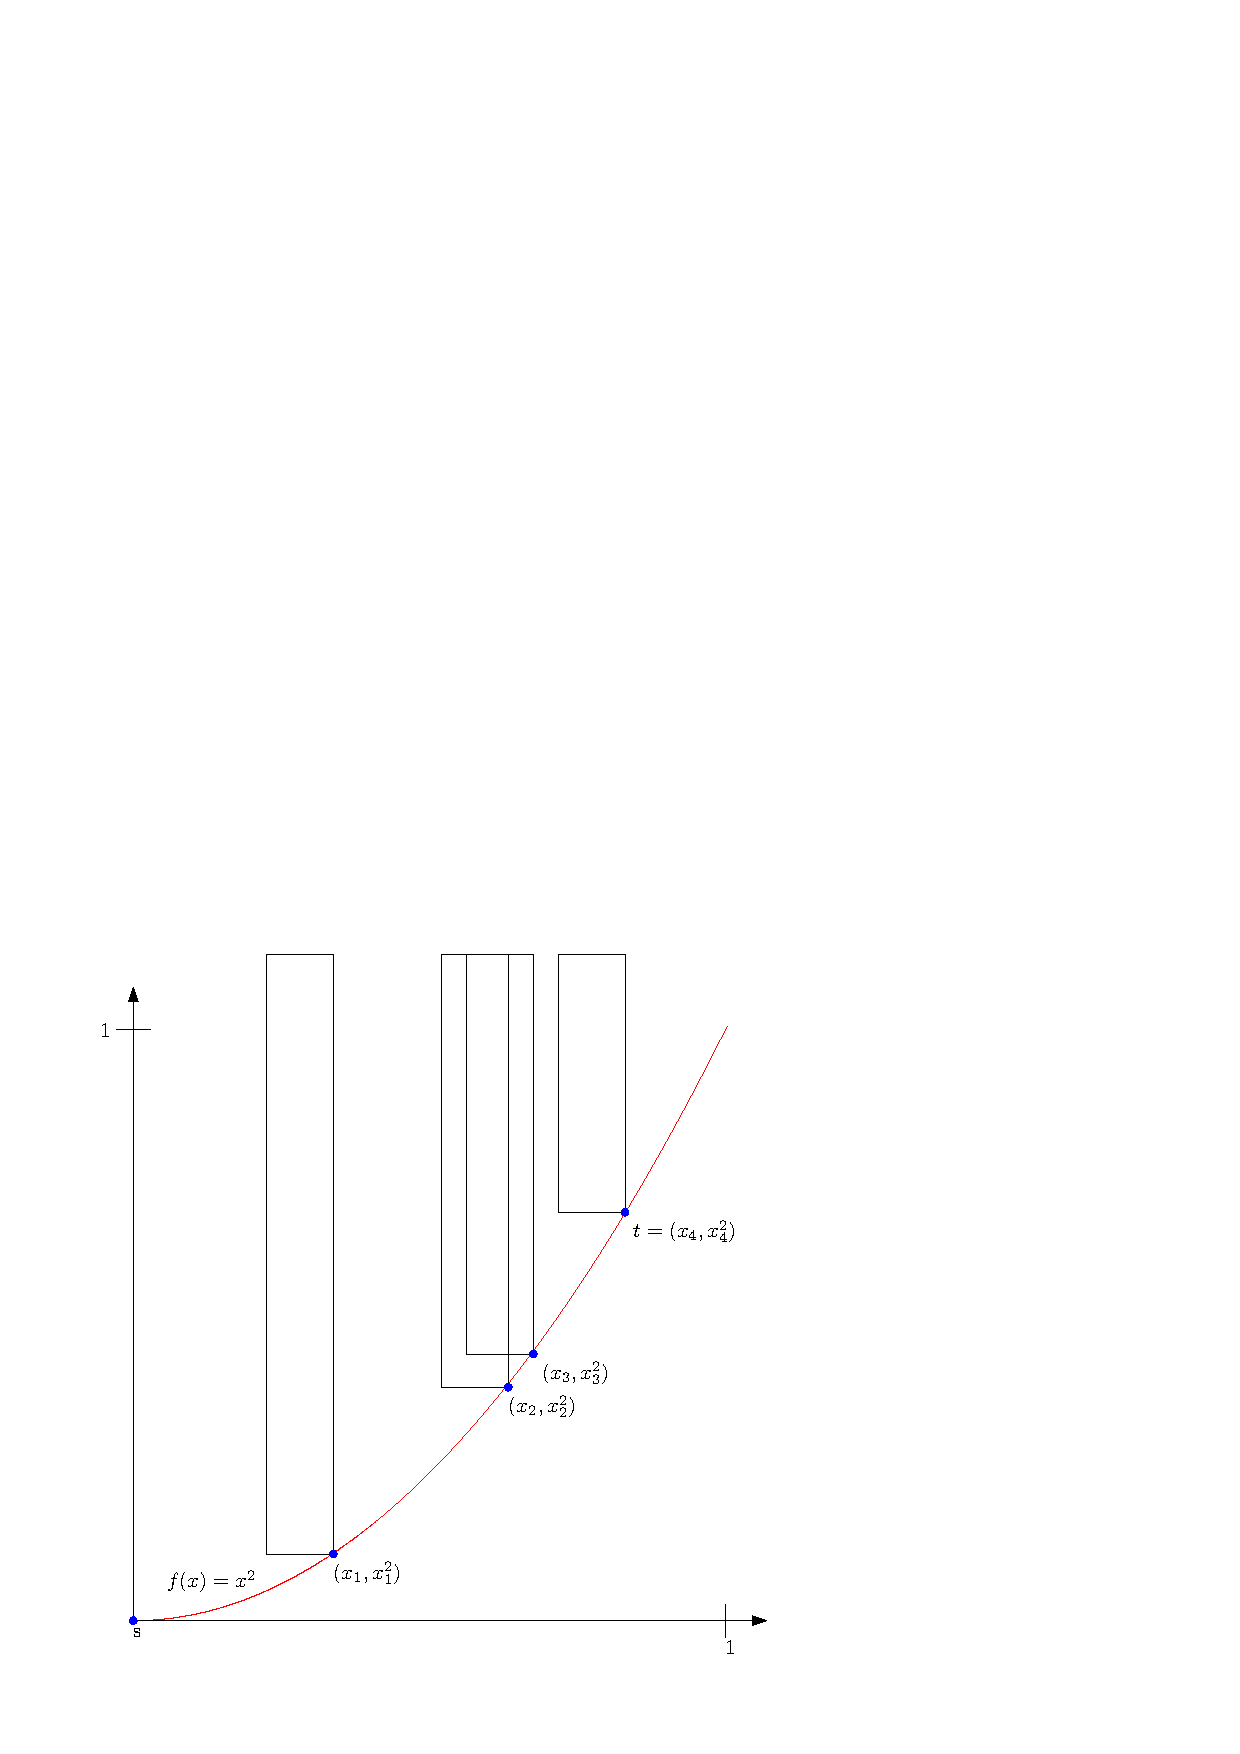
\includegraphics{figures/reduction.pdf}
	\caption{An example of the reduction from sorting numbers to shortest path}
	\label{fig:reduction}
\end{figure}

Set $s=(0,0)$ and let
$i_{max}=\underset{i}{\arg\max}(x_i)$ and set $t=(x_{i_{max}},x_{i_{max}}^2)$.
This gives us an instance of shortest path problem in the plane with obstacles where
each rectangle has the lower right corner laying on the
function $f(x)=x^2$. 

This function is convex which results in every lower right corner of the
rectangles to be visited on the way from $s$ to $t$. Now we can run our SPM
algorithm, to get a path which will be the sorted range of the numbers.

Given that the reduction (constructing the rectangles and finding $t$) takes
$O(n)$ we can conclude that we can make a reduction from number sorting to
finding the shortest path in the plane with obstacles. This mean that we have
shown an $\Omega{(n\log n)}$ lower bound on shortest path in the plane with obstacles.
